\documentclass{scrreprt}

\usepackage{amsmath}
\usepackage{graphicx}
\usepackage{listings}
\usepackage{color}
\usepackage[margin=0.5in]{geometry}
\usepackage{hyperref}
\usepackage{tabularx}
\usepackage{fancybox}


\graphicspath{{./figures/}}

\newcommand{\newtilde}{$\sim$}
\newcommand\tab[1][1cm]{\hspace*{#1}}
\newcommand*\rot{\rotatebox{90}}
\newcommand{\degree}{$^\circ$}

\newcommand{\version}{0.1.0}
\newcommand{\releasedate}{May 23, 2017}

\cornersize{1}


\title{
	Gremm Tunnels \\
	\large A game of wicked multitasking
}

\author{Hunter Damron}
\date{\releasedate}

\begin{document}
	% Title Page
	\maketitle
	
	% Copyright info
	\null\vfill
	\noindent
	Gremm Tunnels - Game Design Document \\
	Version \version, \releasedate \\
	Copyright 2017 - Hunter Damron \\
	\newpage

	% Table of Contents
	\tableofcontents
	\newpage
	
	\chapter{Overview}
		Gremm Tunnels is a puzzle game in which the player controls an army of gremlins through a swamp cave in an attempt to find the exit. What begins as a single gremlin expands quickly into a chaotic mob as the player navigates through various rooms and obstacles. Walls reflect gremlins while mirrors cause gremlins to divide into two - one which passes through and another which reflects off. Each move can cause many results simultaneously so the player must multitask across multiple fronts. Gremm Tunnels arises from simple logic rules but forms a complex system of movement. Gremm also has an emergent series of patterns which define gremlin movement in various ways. Although Gremm Tunnels is a simple game at its heart, it expands to much more than that. The logic is simple and standardized, but with any slight deviation of focus, the results can be unexpected. 
	
	\chapter{State of Art}
		
		\section{Maze/Puzzle Games}
			Gremm Tunnels has been called a puzzle or maze game by many players although none know any games exactly like it. Gremm Tunnels has rightfully gained reputation as a puzzle game since it poses a difficult challenge with the solution as the only reward. With a minimalist art style, Gremm Tunnels focuses on mechanics rather than forming an aesthetic.
			
		\section{Logic Simulation - Conway's Game of Life}
			Like Conway's Game of Life, Gremm Tunnels uses simple logic rules to constrain the movement of gamepieces. Gremm is intended as a game rather than a simple simulation because the player has some control over the situation. The simple rules in Gremm Tunnels were found to create unexpected patterns of movement like those in the Game of Life. These patterns may be usable for more than just a puzzle game.
		
		\section{Differentiation}
			Gremm Tunnels is indeed a puzzle game and shared many characteristics with other puzzle games, but Gremm's primary mechanic of multitasking separates it from other games. Unlike many puzzle games, the player must pay attention to all aspects of the game at all times because each action causes multiple results. The requirement of the player to control various gamepieces simultaneously creates a unique challenge. Gremm Tunnels is differentiated from Conway's Game of life because it has different rules and, more importantly, it permits user input.
	
	\chapter{Specifications}
		\section{System Requirements}
			This game has been tested in Ubuntu 17.04 on Asus hardware. I claim no responsibility for the game's performance on any other hardware or software platform.
		
		\section{Dependencies}
			Gremm Tunnels is written in Python 3.5 and depends on Pygame 1.9.3. Other versions may be satisfactory, but are not officially supported.
			
		\section{Source Code}
			The source code for the digital prototype of Gremm Tunnels available in \autoref{chp:source} and on GitHub at \url{https://github.com/hdamron17/GremmTunnel.git}. Contributions are welcome for both concept ideas and implementation improvements.
	
	\chapter{Game Evolution}
			
		\section{Genesis}
			The idea for the primary mechanic of Gremm Tunnels was created in the attempt to design another game while playing VNA. VNA (Verb Noun Adjective) is a game about creating games where each player must create a game based on a set of three random words: a verb, a noun, and an adjective. The VNA set "double, bakery, glimmering sparked the idea to have the player control two chefs simultaneously to complete tasks, which eventually evolved into the more extreme branching of Gremm Tunnels.
			
		\section{Physical Prototype}
			The first physical prototype was played on an old calendar with lines drawn for doors, walls, and mirrors. Players controlled plastic triangles which had to be moved by hand, a trivial task when only a few are present but a major hassle once they have divided several times. In the physical prototype, mirrors were less frequent, but a counter on each gamepiece also caused division after several moves. This prototype tested various rates of division, several levels of difficulty, and possible collision mechanics.
			
			\subsection{Playtest Reaction}
				The physical prototype was playtested by several members of the game design class. Their reactions were requested in the PMI form which contains one major positive aspect about the game, one major negative, and one proposed change which could possibly make the game better. The responses can be found in \autoref{chp:proto}. The responses varied considerably, but most found the game to be interesting and unique. The counter 
		
		\section{First Digital Prototype}
			The first digital prototype was written in Python using Pygame for graphics. Blue arrows were used as game pieces with black representing free space and white as walls, mirrors, etc.
			
			\subsection{Playtest Reaction}
				The digital prototype was playtested by students at the SC Governor's School. Playtesters were observed during play and questioned after. These are their reactions.
				
				\subsubsection{General}
					Playtesters liked the doubling mechanic and the simple, concise gameplay. For most, it was easy to understand the rules and controls. However, many thought the game was incomplete.
					
				\subsubsection{Suggestions for Gameplay}
					Players requested more immediate feedback for getting nearer to goal. They also thought colored rooms would allow better memorization management because some could not remember which room led where. Although many liked the evil lack of lose condition, some were bothered by it and thought it was too evil. The last suggestion, which was part of the original game plan, is for random map generation with a way of measuring difficulty.
				
				\subsubsection{Technical Issues}
					The basic movements of the game worked successfully, but moving through mirrors and immediately doors caused unexpected bugs due to a design flaw in the new level mechanic. Some doors also malfunctioned, causing strange results in new rooms. Players did not like closing the app in order to restart because many did not know how to or want to navigate the Linux terminal to restart it. The mirror-door issue has not been solved but was temporarily patched by only including doors which are not beside mirrors. The spacebar was added as a restart switch for easier game resets.
			
			\subsection{Game Presentation Reaction}
				After the playtest, the game was presented to mock investors in a project pitch. Investors were afterward invited to play the games to form their opinions. The responses were collected through a form and are included in \autoref{chp:pres}. As in the playtest day for the digital prototype, Gremm Tunnels received positive feedback. Unfortunately, the version presented included more rooms which added to the complexity of the map, leading some players to confusion. In contrast, some players did not struggle at all and thought the game was too short. This difficulty gradient would likely be large in the game because there is no immediate feedback, so such a feedback system would likely improve the game for many players.
				
				\subsubsection{Technical Issues}
					One major issue discovered during the presentation was that some players struggle with the seemingly simple four-key control scheme, likely because players are used to using left and right arrows for movement rather than turning. Another issue which was discovered is that when the player wins and tries to reset the game, they begin in the final room without a reset. The game can be subsequently reset correctly, but this will need to be resolved before distribution.
		
		\section{Miscellaneous Ideas During Development}
			In addition to the game elements which have been included in the game, there have been several notable ideas which have been considered during the evolution of Gremm Tunnels. These ideas have not been rejected but have not been officially accepted either.
			
			\subsection{Random Map Generation and Difficulty Measurement}
				The idea of random map generation has been considered multiple times but each time rejected because of the critical consideration which is required to prepare ideal map layouts. As seen in the playtest sessions, specifically designed map patterns can create purposeful user mistakes, but this would not be possible through automated generation. There has been controversy over this idea because player pitfalls are also often not intended in the map so autonomous map generation could achieve the same stochastic result. One idea which has been considered for difficulty measurement is the A* pathfinding algorithm with slight modifications to measure the number of turns to complete each map. However, a longer path does not always signify a more difficult map so this method would likely not be feasible. The other idea currently pending is to use a modification of the Monte Carlo algorithm to choose random paths through each map layout and determine which percentage of paths end in the correct path. This method may be employed in future generations of the game. 
			
			\subsection{Mirror Counter}
				Although the counter on each gamepiece did not receive positive feedback, is has been suggested that it may be less chaotic to use a single counter which spawns new mirrors on the map over time. This would make the necessity to move efficiently more critical. This mechanic will likely be tested in future prototypes as an additional mechanic.
			
			\subsection{Tunnel Checkpoints}
				Instead of allowing the user to escape completely after each level, future tunnels will likely combine levels by placing checkpoints between each level. In such a system, tunnels will branch and increase in complexity then converge to a single checkpoint room. By converging, players are unable to continue without finding the checkpoint, preventing a previous concern with requiring players to collect items in the maze. However, the player does not truly win until the end of the tunnel. 
	
	\chapter{Mechanics}		
		\section{Goal and Win Condition}
			In each tunnel, one door leads out of the maze. The player has no knowledge of which door leads out or where they start in the maze. They must explore multiple doors to map where each leads until they find the door which ends the game. Currently, the win is displayed only by a screen with the message "You Win - Das Ende," but it will likely be updated when multiple levels are implemented and combined into one large tunnel. The vagueness of the win condition creates the challenge of discovery, 
		
		\section{Lose Condition}
			The current implementation of Gremm Tunnels does not contain a lose condition, but it is still very easy to lose. Because gamepiece collisions can create new walls in the map, these new walls can block the path necessary to win. It is also possible for the player to completely run out of gamepieces and thus be incapable of winning. It is up to the player to determine when they have lost the game by exploring the areas still available. This feature leads to game intensity but also sometimes frustration and will thus likely be reviewed in future versions.
			
		\section{Movement}
			
			\subsection{General}
				Players begin with a single gamepiece which moves in a specific direction denoted by its arrow direction. Through the game, players can acquire more gamepieces which move simultaneously with the original. Instead of moving in the same direction, each piece moves in the direction it is facing. The player can rotate pieces but must rotate all pieces the same direction. Demonstration of the general movement scheme can be found in \autoref{chp:movements}. 
			
			\subsection{Doors}
				Each room in the tunnel is contains doors against its perimeter which connects it to other rooms in the tunnel. Doors point in the direction from which they come and must always be placed against the edge of the map in the current implementation, but may be extended to act as portals which can be placed anywhere on the map in future generations. 
			
				\subsubsection{Room Navigation}
					At the beginning of each level, the player begins in the southern door of a designated starting room. When one gremlin, not necessarily the original, enters a door, that gremlin moves to the room mapped to that exit starting from the opposite side in the new room. All gamepieces except the one which moved to the next room are removed. However, the created walls do not disappear until the player resets the game entirely (this may be replaced by reverting to checkpoints in future maps). Doors are not mapped bidirectionally; thus if a player moves through a door and retreats immediately through that door, they may not end at the same door from which they started. Some doors are not mapped and instead restart the player at the first door in the level. This feature makes the navigation of rooms sightly more difficult and allows for more variety in rooms. 
			
			\subsection{Walls}
				Walls are blocks which cannot be occupied by gamepieces. If a gremlin attempts to move into a wall space, the piece is deflected and returned to its original location in the opposite direction - the equivalent of a rotation by 180\degree. 
			
			\subsection{Mirrors}
				Gremlins moving through mirrors double into two. One gamepiece continues past the mirror while the other, newly created piece moves perpendicularly to the direction of motion as if it had been reflected off the mirror. 
			
			\subsection{Generic Items}
				The game currently does not implement any meaning, but maps can contain circles which represent generic items. These generic items may be implemented in the future as some sort of power up or another movement inhibitor. 
			
			\subsection{Gamepiece Collisions}
				In the case that two gamepieces attempt to occupy the same space, those two pieces are removed from the board and replaced with a new wall. These walls become part of the map until the level is restarted and act like the original walls once they are created. 
			
			\subsection{Recursive Nature}
				In order to prevent gamepieces from inevitably forming walls after dividing within a mirror tile, gamepieces move recursively such that each gamepiece moves forward from the mirror through whichever tile is before it. In the case of adjacent mirrors and/or walls, this causes pieces to move multiple times before arriving at stable locations. This implementation implements this nature recursively, although it could also be implemented iteratively. 

				\subsubsection{Handling Inescapable Movements}
					In some situations, this recursive movement may be inescapable, spawning infinite gamepieces. Naturally, this is not possible for the game to handle. Since each gamepiece must be in a finite number of locations, the recursion is limited to a certain depth and the resulting gamepieces are used. This results in a formation of walls where the gamepieces would recur infinitely. 
			
			\subsection{Emergent Patterns}
				
				\subsubsection{Criteria for Infinite Recursion}
					Although the first tunnel was created without much attention, several patterns have been discovered which can be used to develop more complex maps. First, movements of infinite recursion have been discovered to always occur in scenarios where a mirror is surrounded by two or more mirrors. Future experimentation will be conducted to generalize the pattern for multiple adjacent mirrors. 
				
				\subsubsection{Turing Completeness}
					During the playtesting stage, it was noted that the logic of Gremm Tunnels may be Turing complete and thus capable of use as an obscure but viable programming language. The game possesses the logic necessary because movement branches during mirrors conditionally. This document makes no claim of the validity of Gremm Tunnels as a programming language, but the possibility will be explored and possibly exploited in the future of the game.
	
	\chapter{User Interface}
		
		\section{Controls}
			Gremm Tunnels is controlled by only four keys: the spacebar and up, left, and right arrows. Because the player controls gamepieces moving in different directions, it is impractical to move in the direction of the arrow, so Gremm Tunnels uses a different layout than similar games. Left and right arrows rotate all gamepieces counterclockwise and clockwise, respectively. The up arrow then moves all gamepieces in the direction they are pointing. Because the game is difficult to win, the spacebar is used to quickly restart the level. In future generations of the game, there would likely be a slightly more complex keyboard layout to incorporate other features like power up use and menu navigation. However, it is planned to keep the control scheme as simplistic as possible. 
		
		\section{Display}
			The current implementation of Gremm Tunnels uses a simplistic, geometric graphical theme. The board is represented as a board of squares with each square a possible location on the map. Empty squares are black while occupied squares are filled by the color of the map. By popular demand, each room of the tunnel is designated a specific color to allow players to more easily memorize the room layout. Doors are represented by triangles which occupy one fourth of a square and point in the direction of the door. Diagonal lines indicate mirrors which lie across the square in the direction of either a forward or back slash. Gremlins are implemented as blue arrows which lie above the background square. When directed, they move in the direction they point. Although their functionality is not yet implemented or decided, generic items which may represent power ups in the future are represented by circles. The game is preceded by a very brief direction message and followed by another short message on winning. Map examples can be seen in \autoref{chp:rooms}.
		
		\section{Menu Navigation}
			Although only a single level is currently implemented so there is no need for navigation menus, future generations of the game are planned to include a simple menu to allow players to move to checkpoint locations through the explored area of the map. 
		
	\chapter{Aesthetics}
	
		\section{Minimalist Style}
			Although the original game was developed more closely centered around the gremlin theme, the game has evolved as more of a simplistic puzzle game. The current implementation does not employ any artwork other than geometric shapes for the sake of programmatic simplicity, but this minimalist style has been adopted. Simple design encourages the feeling of a puzzle game rather than an exploration game which is better suited for Gremm Tunnels. The lack artwork employed by Gremm Tunnels also conveys an isolation between the player and the game such that players are against the game rather than in the game. 
		
		\section{Future Aesthetic Goals}
			Because the first implementation focused on settling the mechanics of Gremm Tunnels, aesthetics have not been properly considered. Although the story of Gremm Tunnels has been mostly deprecated, the game may use the theme for art or sound in order to create a mysterious mood. Sound and art may also be used in future implementation to help convey game information. For example, background art may contain more light or music may play at a faster pace when the user nears the end of the tunnel. This would allow the aesthetics and mechanics to merge in a way which makes gameplay more fluid.
		
	\chapter{Market Strategy}
		
		\section{Target Market}
			Although not the original intent, this game is primarily a puzzle game for intuitive minds which seek challenge. The game is unforgiving in many aspects, a large appeal for many players and a fatal flaw for others. On the Bartle scale for player types, this game tends to appeal to explorers who play for the sake of discovery. It may also appeal to achiever types because of the joy of winning, but winning currently is not rewarded by more than the excitement of escaping. Although simple, the game is also ideal for players with logical skills and the ability to combine simple truths into complex systems because Gremm Tunnels is itself a complex system produced by basic rules. Gameplay keeps players almost always on the edge of frustration which makes it effective as a puzzle game but annoying for players with low tolerance for losing. Gremm Tunnels requires a mixture of perseverance and the ability to quit when the game is no longer possible. Although the market has not been tested extensively, these qualities will likely be found in adults and students who expose themselves to math or logic puzzles regularly. 
		
		\section{Path to Market}
			This game was not conceptualized for the market, so this path has not been planned but may be in the future. Playtesters have commented that Gremm Tunnels is unique in many aspects so the possibility of a market distribution will likely be explored. 
		
	\chapter{Future Work}
		Much of the future of Gremm Tunnels has been mentioned throughout this document because it spans all areas of the game. The current implementation of Gremm Tunnels is a digital prototype for a game which could take multiple paths from where it is. This section provides a summary of the work which could be done to make Gremm Tunnels more complete.
		
		\section{Conceptual}
			While the game can be played in a way which feels complete, there is still work to be done. The game currently becomes stale once the player either recognizes the patterns and is able to solve levels trivially or is unable to succeed and becomes overly frustrated. The skill-difficulty curve will need to be adjusted accordingly through map development. Thus, a method of judging map difficulty will also need to be developed in order to effectively create maps. To prevent staleness, the generic item entity may be employed as a mechanism to temporarily modify the rules and allow a change in gameplay.
		
		\section{Technical}
			The basic mechanics of Gremm Tunnels are concrete and will likely not change, but they currently contain several conflicts which have not yet been addressed. These missing pieces occur mostly at obscure boundaries and can be avoided, but they will need to be resolved before Gremm Tunnels can be considered entirely functional. One major concern is the handling of doors with adjacent mirrors. These cause problems because of the recursive implementation, a design choice which will likely need to be replace with an iterative solution. Doors placed in corners may also cause issues because there is no officially supported decision about which direction to face the door. Until they are resolved, both issues can be avoided with constrained door placement. 
			
			In addition to the design choices which must be made, more maps must be created using the knowledge of patterns discovered during playtesting to exploit user pitfalls proportionately to intended difficulty. 
		
	\chapter{Shoutouts}
		Shoutout to Python and Pygame for a simple graphics development environment and amazing software in general. 
		
		Shoutout to classmates Victoria Young, Pierce Carrouth, Dennis Perea, and Daved Schmitt for extensive playtesting and opinions. 
		
		Shoutout to the rest of the official playtesters for useful feedback and bug discovery.
		
		Shoutout to Dr. Al DeGennaro for the Game Design Course, the birthplace of this project.
		
	\chapter{Author}
		Hunter Damron is a current senior at the South Carolina Governor's School for Science and Math. Gremm Tunnels was created as the capstone project for his Game Design course with Dr. DeGennaro. Hunter plans to major in computer engineering and possibly minor in Math at the University of South Carolina in Columbia. Hunter has experience in many aspects of computer science and math, but this project is his first dive into game design. Although he does not play many games, Hunter is an explorer type player who enjoys learning about his environment and the possibilities of the game more than completing the game in the intended way. Hunter created this game with the same idea that a simple game would allow possibility for discovery. He allowed the game to develop with an evil nature purely for the enjoyment of watching players struggle and was surprised by the positive results. Although this game was a class requirement, Hunter may continue development on the project because of its success among his teachers and classmates. 
	
	\appendix
	
	\chapter{Tunnel Room Examples}\label{chp:rooms}
		\begin{figure}[!ht]
			\centering
			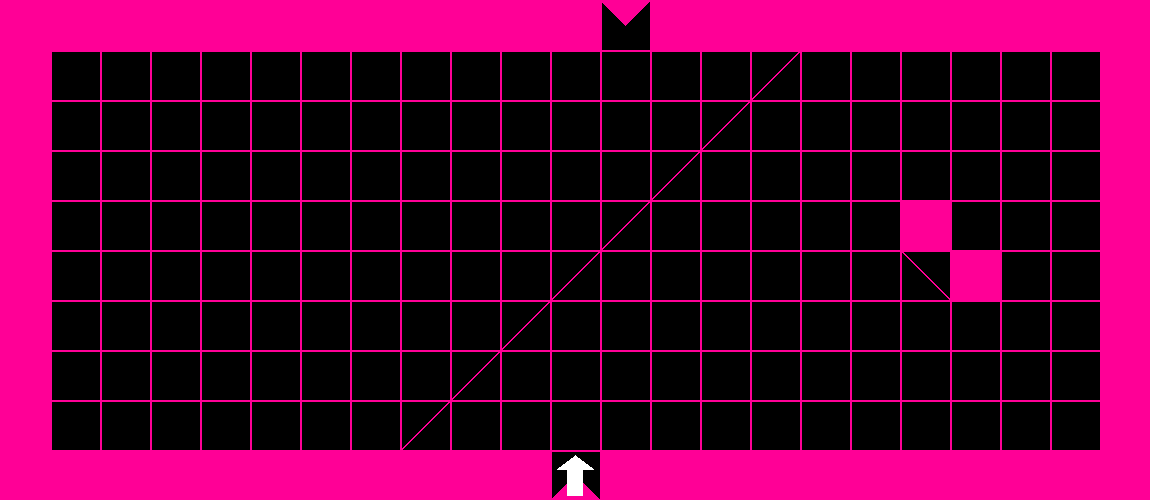
\includegraphics[width=\columnwidth]{start}
			\caption{First room to allow players to acquaint themselves with the map}
			\label{fig:start}
		\end{figure}
	
		\begin{figure}[!ht]
			\centering
			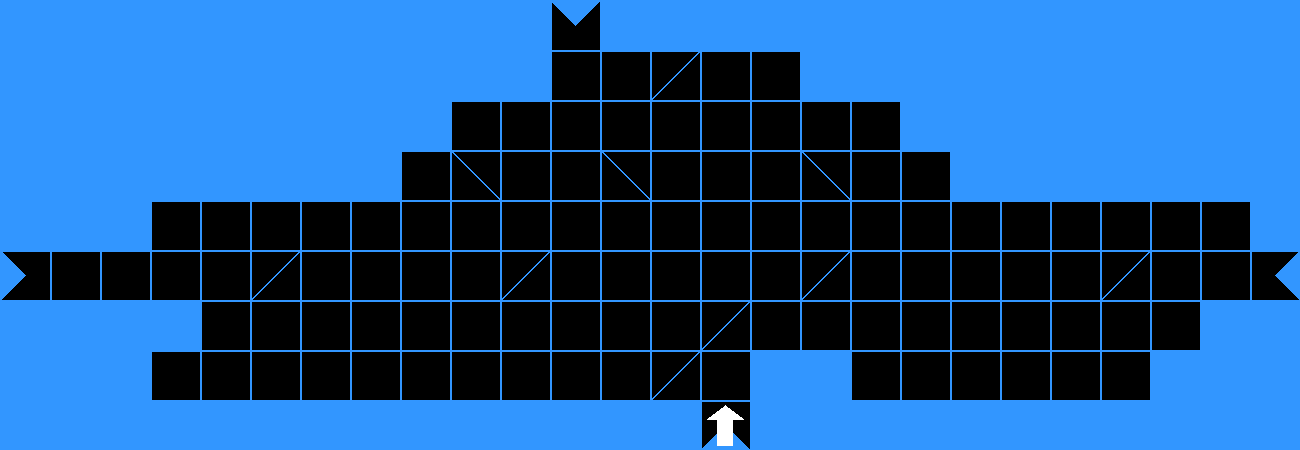
\includegraphics[width=\columnwidth]{easy}
			\caption{Easy difficulty room}
			\label{fig:easy}
		\end{figure}
	
		\begin{figure}[!ht]
			\centering
			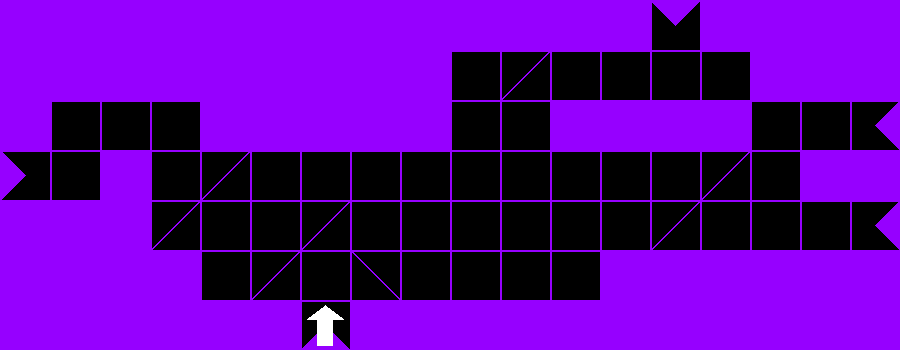
\includegraphics[width=\columnwidth]{medium}
			\caption{Medium difficulty room}
			\label{fig:medium}
		\end{figure}
	
		\begin{figure}[!ht]
			\centering
			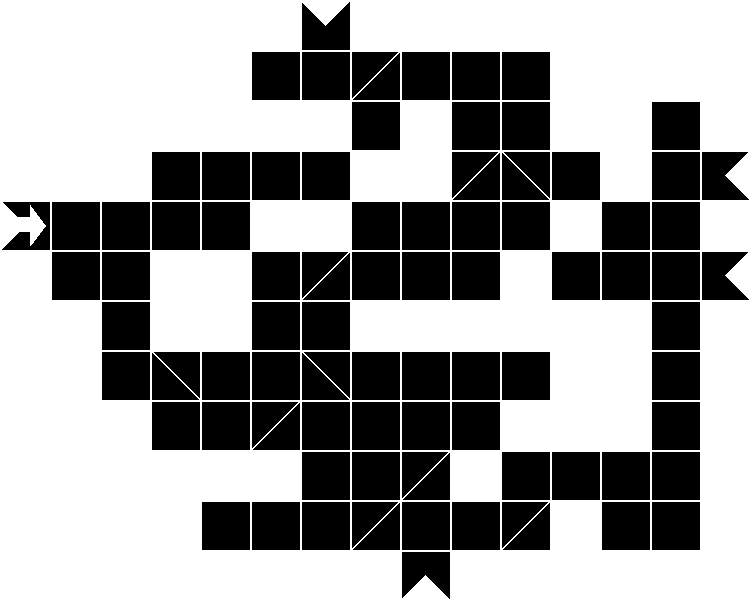
\includegraphics[width=\columnwidth]{hard}
			\caption{Hard difficulty room}
			\label{fig:hard}
		\end{figure}
	
	\chapter{Movement Examples}\label{chp:movements}
	
		\begin{figure}[!ht]
			\centering
			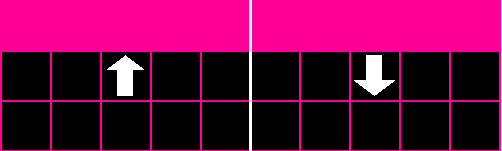
\includegraphics[width=\columnwidth]{wall}
			\caption{Displays total reflection off walls. (Right image shows frame immediately after moving forward from left image.)}
			\label{fig:wall}
		\end{figure}
	
		\begin{figure}[!ht]
			\centering
			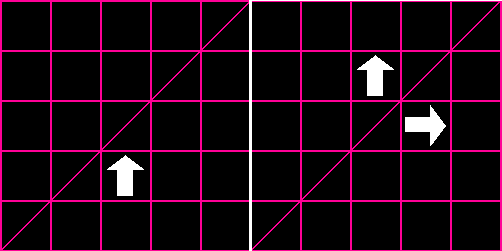
\includegraphics[width=\columnwidth]{mirror}
			\caption{Displays how gremlins react to moving through mirrors by partially reflecting. (Right image shows frame immediately after moving forward from left image.)}
			\label{fig:mirror}
		\end{figure}
	
		\begin{figure}[!ht]
			\centering
			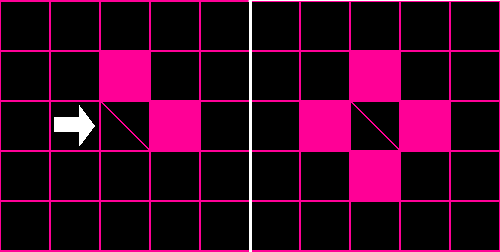
\includegraphics[width=\columnwidth]{deathtrap}
			\caption{Displays how certain room configurations can be impossible to navigate through. (Right image shows frame immediately after moving forward from left image.)}
			\label{fig:deathtrap}
		\end{figure}
	
		\begin{figure}[!ht]
			\centering
			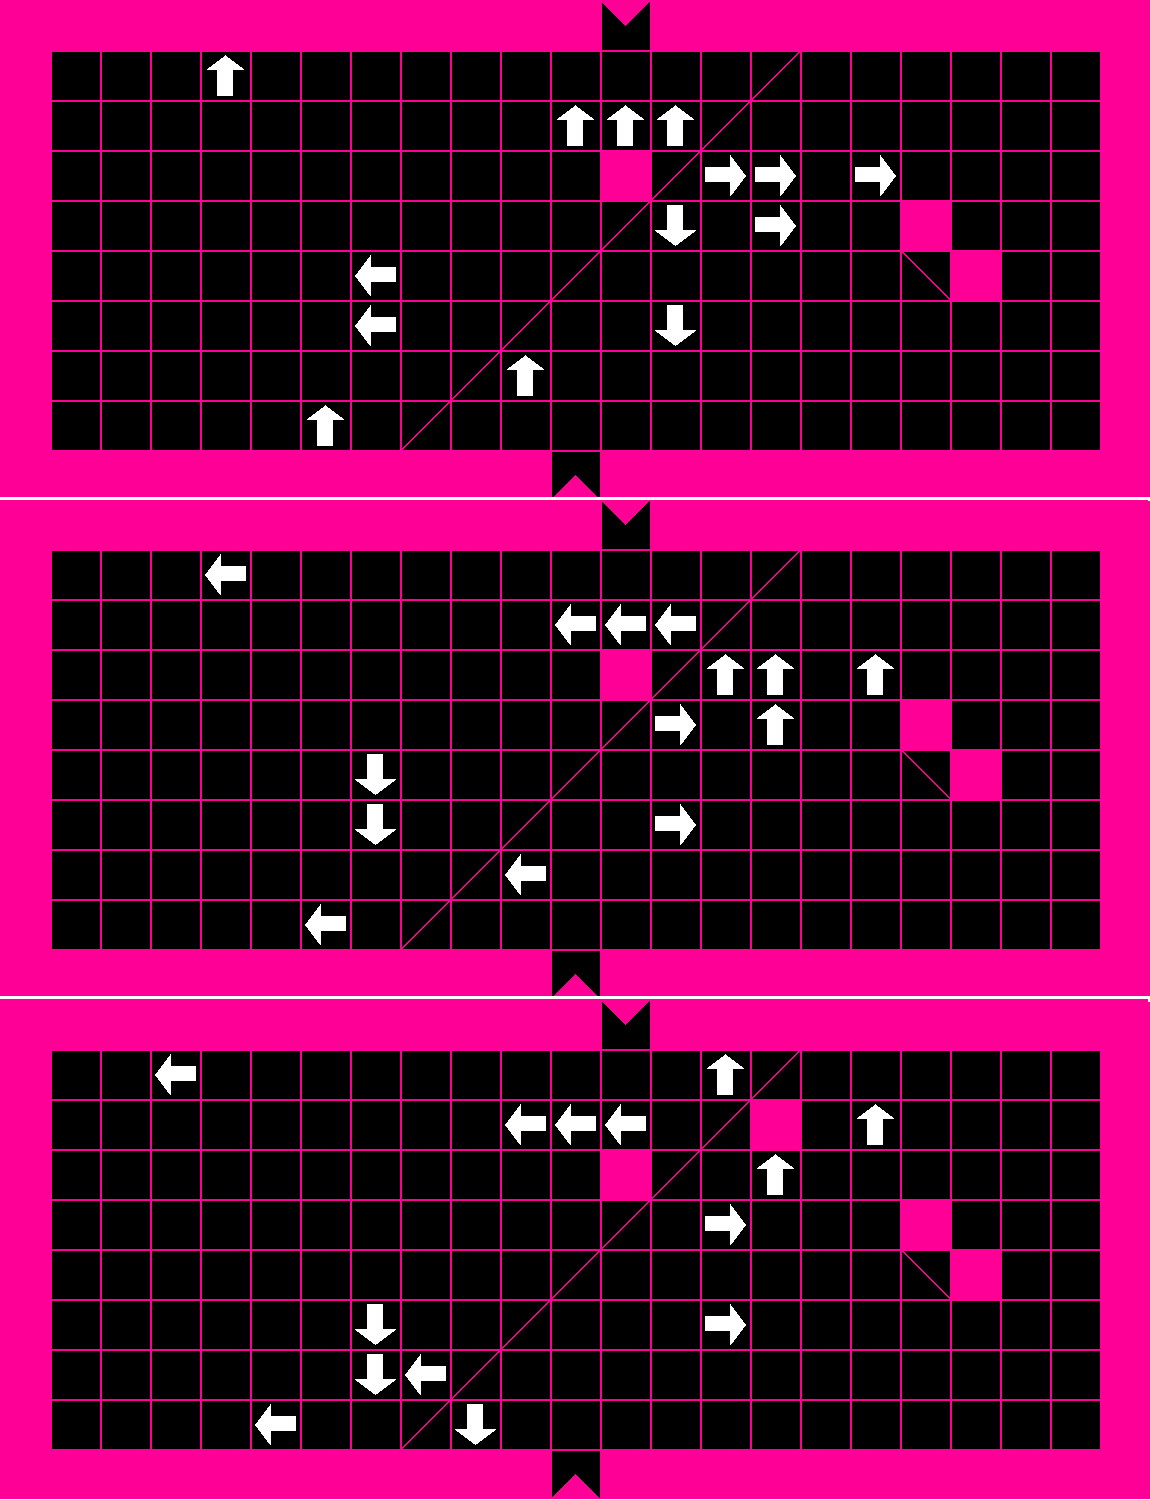
\includegraphics[width=\columnwidth]{multi}
			\caption{
				Demonstration of movement with multiple gremlins.
				Top: Initial frame containing multiple gamepieces acquired from moving multiple times through mirrors.
				Middle: Game configuration after pressing left key to turn counterclockwise.
				Bottom: Game configuration after pressing up key to move forward.
			}
			\label{fig:multi}
		\end{figure}
	
	\chapter{Physical Prototype Feedback}\label{chp:proto}
		\begin{quote}
			Plus: Your game is very interesting, controlling multiple gremlins at the same time makes the game unique and fun.  I especially love how when gremlins collide, they explode the board.  The theme of Gremlins is also very cool, and the usage of mirrors creating more Gremlins is a very clever mechanic.
			
			Minus: I feel the game could use harder levels or something that truly punishes the player.  I feel that when I play your game, I do not get punished at all for making mistakes. Furthermore, even though it was a prototype, moving the counters over and over became annoying.
			
			Interesting: I feel that the theme of your game, which is gremlins trying to collect gems?  (I forgot) and then trying to get out is really cool.  One idea I feel you could incorporate is rewarding the player based off of how many gremlins he is able to get out, which would encourage players to create more gremlins and be more cautious with their decisions.
			
			\hfill\newtilde Dennis Perea\\
		\end{quote}
		
		\begin{quote}
			Plus: The game was not too difficult and fairly easy to understand once I got the hang of it.
			
			Minus: It was almost too easy, and it seemed like it could get boring quickly if there was not enough variability in feedback.
			
			Interesting: I like the idea of multiplying, but the win condition should be smaller or harder. I also think it'd be interesting to have a couple semi-autonomous "bad" gremlins. Also, collisions must be dealt with. Something that'd be interesting is having 2 players compete to collect coins and when 2 gremlins meet, they fight each other. 
			
			\hfill\newtilde Victoria Young\\
		\end{quote}
		
		\begin{quote}
			Is it a puzzle game? If so, I don't think it can survive on this mechanic alone. 
			
			\tab\tab Other elements are clearly needed to carry the player's interest along. I think the counter really limits design possibilities.
			
			Perhaps add mechanics for being yourself more time, then the counter could be more of a "balancing act"
			
			\hfill\newtilde David Schmitt\\
		\end{quote}
	
	\chapter{Presentation Feedback}\label{chp:pres}
		Responses for clarity-fun were completed on a scale 1-7 while the others were free response. The score section was left highly to interpretation so the results were far from standardized. 
		\begin{center}
		\begin{tabularx}{\textwidth}{ |c|c|c|c|c|c|X|X|X|X| }
			\hline
			\rot{Clarity} & \rot{Flow} & \rot{Balance} & \rot{Length} & \rot{Integration \ } & \rot{Fun} & Strength & Weakness & Comparable Games & Score \\\hline
			6 & 6 & 5 & 7 & 6 & 6 & Very difficult and unforgiving & Very difficult and unforgiving & Gru, Zork, Myst & 7/10 \\\hline
			7 & 7 & 7 & 7 & 7 & 7 & What should be & frustrating but makes it fun! & Unique! & 7/7 \\\hline
			6 & & & & & 7 & clever premise & I only have two eyes & & 90\% \\\hline
			7 & 6 & 7 & 7 & 7 & 7 & Intellectually stimulating & & & 41 \\\hline
			7 & 7 & 7 & 7 & 7 & 7 & Very \Ovalbox{fun} & more colors! & nothing ever seen & \\\hline
			7 & 7 & 7 & 4 & 7 & 7 & & Hard to understand at 1st and not obvious how to win & pacman & \\\hline
			6 & 7 & 6 & 6 & 7 & 7 & Fun, food different & glitch after winning & maze solvers & \\\hline
			6 & 7 & 6 & 6 & 5 & 6 & it works & some levels can't be beat. no end goal & & 36 \\\hline
			6 & 6 & 6 & 3 & 6 & 7 & very simple, easy & a little short & escape goat, that one Atari & 34 \\\hline
			3 & 5 & 7 & 6 & & 6 & Kind of endless, many approaches & confusing instructions & & \\\hline
			6 & 6 & 5 & 7 & 6 & 7 & & & & \\\hline
			7 & 7 & 7 & 7 & 7 & 7 & concise, simple, focused & graphics aren't "the best" and not enough levels & portal? any puzzler & 49 \\\hline
		\end{tabularx}
		\end{center}
	
	\chapter{Map and Layout Source Files}\label{chp:map-files}
		
		\lstset{
		language={},
		breaklines=true,
		numbers=none
		}
		
		\section{gbd1.layout}
			\lstinputlisting{py_src/assets/gbd1/gbd1.layout}
		
		\section{start.map}
			\lstinputlisting{py_src/assets/gbd1/start.map}
		
		\section{easy.map}
			\lstinputlisting{py_src/assets/gbd1/easy.map}
		
		\section{medium.map}
			\lstinputlisting{py_src/assets/gbd1/medium.map}
		
		\section{hard.map}
			\lstinputlisting{py_src/assets/gbd1/hard.map}
	
	\chapter{Source Code}\label{chp:source}
		\lstset{
			basicstyle=\ttfamily,
			language=Python,
			breaklines=true,
			otherkeywords={self},
			keywordstyle=\color{blue}\ttfamily,
			stringstyle=\color{red}\ttfamily,
			commentstyle=\color{green}\ttfamily,
			morecomment=[l][\color{magenta}]{\#},
			numbers=left
		}
	
		\section{gremm\_tunnel.py}
			\lstinputlisting{py_src/src/gremm_tunnel.py}
		\section{general.py}
			\lstinputlisting{py_src/src/general.py}
		\section{engine.py}
			\lstinputlisting{py_src/src/engine.py}
		\section{gui.py}
			\lstinputlisting{py_src/src/gui.py}
		\section{gameboard.py}
			\lstinputlisting{py_src/src/gameboard.py}
		
\end{document}